
%%%%%%%%%%%%%%%%%%%%%%%%%%%%%

%编译请在README.tex下编译！
%如未阅读README.tex，请先阅读README.tex

%%%%%%%%%%%%%%%%%%%%%%%%%%%%%
\chapter{学习指南手册编辑说明}
\section{项目简介}
\begin{introduction}
    \item 写作目的
    \item 文档结构
    \item 文章对应内容的结构
\end{introduction}

\begin{notebox}
    该部分不是原版elegantbook的结构，我希望写一点总结性的内容，因此添加了这样一个方框。
\end{notebox}

\begin{presentbox}
    这个是一个简单的展示框，只有蓝色描边哦~
\end{presentbox}
本项目是一个基于 \textbf{ElegantBook} 模板的 LaTeX 文档工程，涉及生命学院诸多的活动\footnote{这是一个注脚，方便在有需要的地方添加独立于正文的备注和说明}：
\begin{itemize}
  \item 竞赛
  \item 交流实习
  \item 申请：
  \begin{itemize}
      \item 出国
      \item 保研
  \end{itemize}
\end{itemize}

\textbf{README.tex目标读者：} 后续接手编辑本项目的同学 / 合作者 

\textbf{本文的目标：} 在项目交接的过程中，我们发现由于原书内容繁杂、格式颇多，因此提供一个文档，最小化实现以及编译该书的不同结构，帮助合作者用最短时间上手修改并正确编译文档；了解编辑本书的核心要义。

\textbf{使用方法：} 在该\LaTeX 文档下，对照相应章节结构，添加、编辑或者删除对应的的篇章部分即可。

\newpage

\section{文件结构说明}

项目的核心结构如下：
\begin{verbatim}
project/
|-- main.tex        % 正式文档（最终输出 PDF）
|-- README.tex      % 本说明文档
|-- mian.cls        % 配置文档，请在此处添加必要的包，注意解决冲突问题！
|-- chapters/       % 如需添加或者删除章节，请在此文件夹下新建
|   |-- 
|   |-- 竞赛.tex
|   |-- 交流.tex
|   |-- 保研.tex
|   |-- 申请.tex
|   |-- 经验贴合集.tex
|-- figure          % 储存封面图片
|-- image           % 储存文件中的图片
|-- pdf             % 某些以pdf格式插入的图片，就放在这里了
|-- reference.bib   % 个人没用到引用，但是还是放在这里了
|-- License         % elegantbook的License
\end{verbatim}

\section*{重要说明}
\begin{remark}
\begin{itemize}
  \item \textbf{main.tex} 是文档入口，在此文档下编译该书！
  \item \textbf{README.tex} 仅用于说明和示例，不会被 main.tex 引用。
  \item 各章节文件位于 \texttt{chapters/}，不要在其中写导言区！请注意，在chapters中添加章节后需要在正文对应的章节位置添加：
\begin{lstlisting}
\input{chapters/'章节名'}
\end{lstlisting}
\end{itemize}
\end{remark}
\section{文章组织思路以及征稿要求}

\notetitle{组织框架与征稿要求}
%这个标题会好看一点，但是没法显示在目录里面，所以会有两个目录，不需要担心会不会重复这个问题

首先关于本书结构，我的构想是把整份指南做成“双入口模式”的结构：目录以及正文按读者最关心的主题拆分成相对独立的模块（例如竞赛、交流、申请过程中的材料与面试），适合目标明确、想直达某一部分的人；同时，为了避免读者被章节顺序束缚，再提供一个时间入口的框架，详细罗列不同时间段内可以完成的内容，可以辅助明确自己所在的状态，了解下一步应该做什么。

其次，关于对外征稿与内容定位上，我会明确本指南以“经验”作为核心材料——尽量提供可复用、可落地的做法与细节；但同时也强调“思考”同样重要，因为经验若缺少对规则、边界与选择逻辑的提炼，往往只能复制表面操作、无法迁移到不同背景与不同时间点，因此每个经验片段都会尽量对应到一条更通用的判断原则，帮助读者真正理解并形成自己的决策能力。

\section{文档必要结构以及内容}
\subsection{图片、公式与引用}

\subsection{插入}

插入一张单独的图片：
\begin{lstlisting}
\begin{figure}[H]
    \centering
    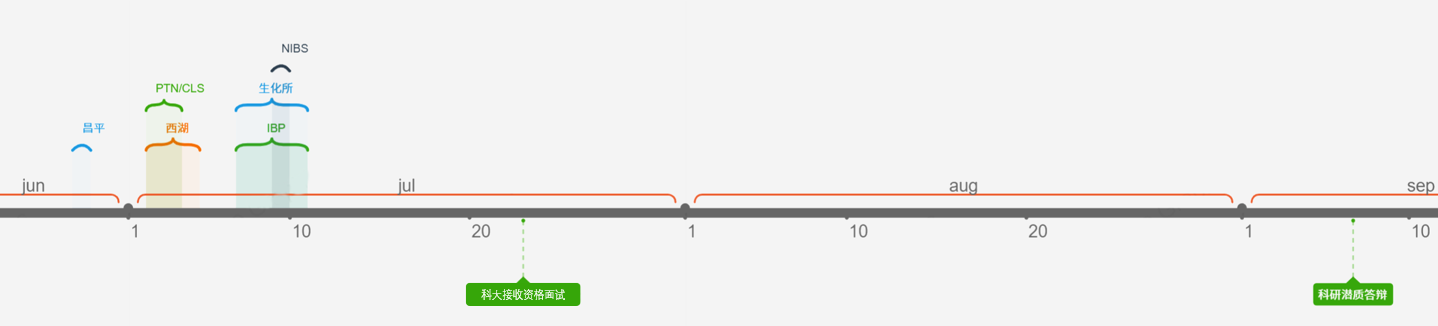
\includegraphics[width=0.95\textwidth]{image/学业指南/夏令营/夏令营timeline.png}
    \caption{夏令营list}
\end{figure}  
\end{lstlisting}

插入两张呢？
\begin{lstlisting}
\begin{minipage}{0.44\textwidth}
  \centering
  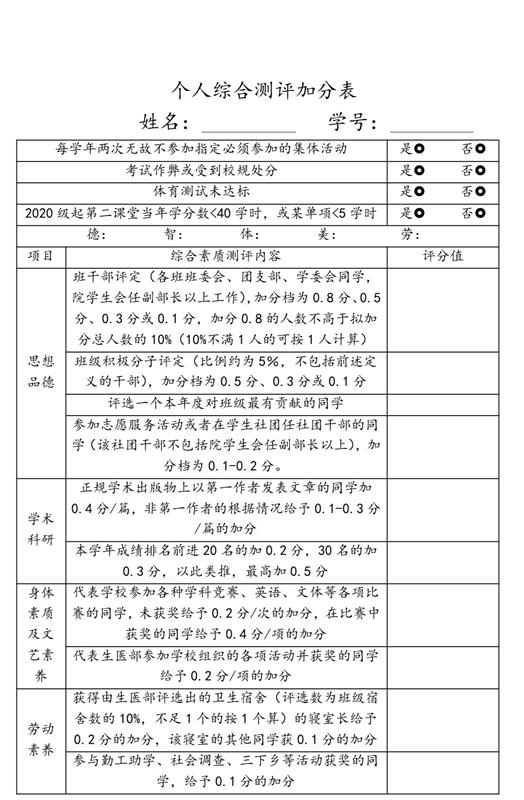
\includegraphics[width=0.88\textwidth]{image/学业指南/学业/个人综测加分表.jpg}
\end{minipage}
\hspace{1em}
\begin{minipage}{0.45\textwidth}
  \centering
  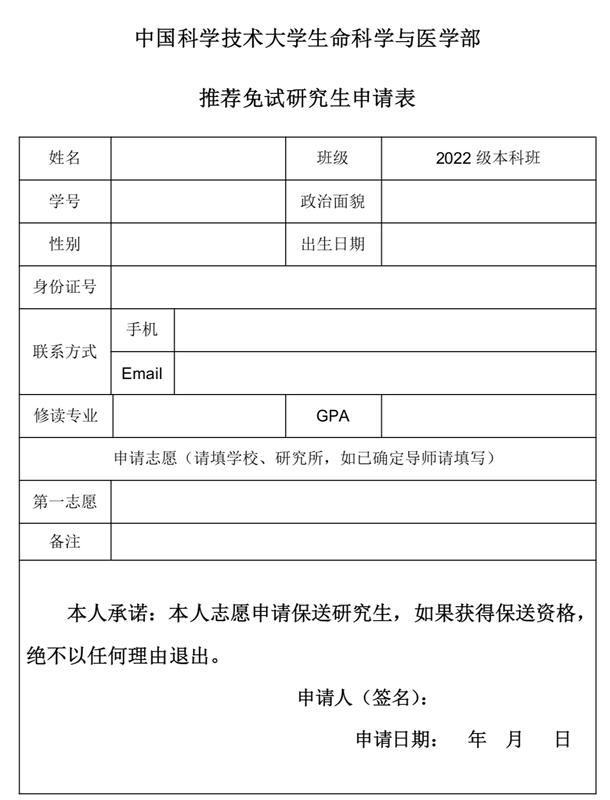
\includegraphics[width=0.88\textwidth]{image/学业指南/学业/外推资格申请表.jpg}
\end{minipage}
\end{lstlisting}

如果要插入一个pdf呢？

\begin{lstlisting}

\includepdf[pages=-]{pdf/NIBS.pdf}
\end{lstlisting}
如要指定页面的话，就改成：

\begin{lstlisting}

\includepdf[pages=1-2]{pdf/NIBS.pdf}
\end{lstlisting}

如果想要插入超链接的话，使用：
\begin{lstlisting}
\href{vista.ustc.edu.cn}{全球化学习平台}
\end{lstlisting}

\subsection{公式、化学式等}

这个大抵不需要吧，就按照正常的\LaTeX 的公式插入方法即可。

\begin{lstlisting}[language=TeX]
\begin{equation}
E = mc^2
\end{equation}
\end{lstlisting}
化学可能略显复杂，支持mchm以及chemfig，mchm用于书写普通化学式、chemfig用于书写有机化合物。其中mchm：

\begin{lstlisting}[language=TeX]
\ce{Na+}   %无需上下标，可以自动识别
\end{lstlisting}
编译结果：
\ce{Na+} 

\section{常见问题（FAQ）}

\subsection*{Q1：这个文件需要怎么运行}
\begin{itemize}
  \item 作者在学校 \LaTeX 线上平台运行
  \item 曾经尝试在本地实现，但是出现字体等bug，未继续尝试本地版。
\end{itemize}

\subsection*{Q2：可以同时有 main.tex 和 README.tex 吗？}
可以。它们是两个\textbf{独立的可编译入口文件}，互不影响。

\section*{Q3：不熟 LaTeX 怎么办？}
\begin{itemize}
  \item 本文就是为了辅助不太熟悉\LaTeX 的同学，请对照源代码以及pdf文件，尽量模仿已有章节写法
  \item 如果不熟悉，请不要随意改cls文件，史山代码千万别乱碰。
  \item 注意定时备份，一版不超过10M，不用担心内存问题。
\end{itemize}

\section*{结束语}

如果你能看到这里，说明你已经具备独立编辑本项目的能力了。如有不确定之处，请联系项目维护者或在 README 中补充说明。